%\documentclass[10pt,a4paper]{article}
\documentclass[letterpaper,10pt,draftclsnofoot,onecolumn]{article}
\usepackage[letterpaper, margin=.75in]{geometry}

\usepackage{hyperref}
\usepackage{listings}
\usepackage{wasysym}
\usepackage{graphicx}

\graphicspath{ {./images/}}

\hypersetup{
	colorlinks,
	citecolor=black,
	filecolor=black,
	linkcolor=black,
	urlcolor=black
}
\begin{document}

\begin{titlepage}
\vspace*{\fill}
\begin{center}
{\Large Tut-Tut, The IoT Rain Fall Detector Final Hand Off Document}
\\[0.3cm]

{\large CS 461 - Spring 2019}
\\[0.3cm]

{\large Jonathan Rohr}
\\[0.3cm]

{\large Michael Gillett}
\\[0.3cm]

{\large Shreyans Khunteta}
\\[0.3cm]

{\large June 1st, 2019}
\\[1cm]

{\Large Abstract}
\end{center}
Tut-Tut, the IoT Raindrop Detector, is a project under the domain of the OPEnS (Openly Published Environment Sensing) Lab at Oregon State University. Tut-Tut will be able to detect a raindrop of any size, get an idea of the drop's mass from the intensity at which it falls, and detect the frequency of raindrops. After Tut-Tut gathers this data, it will be able to wirelessly transmit the information to a central server and communicate it to other IoT devices around Oregon State University. The detector will periodically wake up to check for rain and will stay awake as long as rain is detected within two minutes. If it does not detect raindrops within two minutes, it will go back to sleep. As a stretch goal, we will design an online mobile application to which the physical device will transmit information about the raindrops. If this stretch goal is not met, then the data will be stored in a Google Sheet.
\vspace*{\fill}
\end{titlepage}

\tableofcontents

\pagebreak

\section{Introduction}
In this document we will be outlining the requirements of Tut-Tut, the Internet of Things (IoT) Rainfall Detector. Requirements are as per requested by Chet Udell and the OPEnS Lab located at Oregon State University.

\subsection{Requested By Who and Why}
This project was requested by Chet Udell, on behalf of the OPEnS Lab at Oregon State University. The OPEnS Lab at Oregon State University is dedicated to developing technologies that increase our knowledge of the world we live in. They develop tools that can for example, detect the water content of soil across a patch of farm land, and give real time updates about their conditions. If the field is getting too much water in one particular area, their technology could tell the the sprinkler system in that area to start watering  the sections of the field in desperate need of water based on the water content readings.

\subsection{Team members and roles}
The members of this team were Jonathan Rohr, Michael Gillett and Shreyans Khunteta.  Jonathan focused primarily on the microcontroller and coding. Michael focused primarily on 3D printing and designing the physical casing. Shreyans also focused on 3D printing as well as being the primary writer of documentation. However, all members of the team participated somewhat in most aspects of the project and all members communicated their tasks and how to do them with one another. This was so that if one person was unable to complete that task, someone else would be able to pick it up. 

%\tableofcontents
\begin{center}
\begin{tabular}{ |p{0.3\linewidth}|p{0.3\linewidth}|p{0.3\linewidth}| }
\hline
\multicolumn{3}{|c|}{Requirements Doc Revisions Table} \\
\hline
Section & Original & New \\
\hline
Overall &
Previously, this document consistently stated that Tut-Tut would be capable of measuring the specific mass of a raindrop. &
Now this document has changed all references to mass by replacing them with references to raindrop impact and intensity. Ultimately finding the specific mass of a raindrop was deemed out of scope for this project. \\
 & \\
2.2 &
The main functions of this raindrop detector are that it can detect raindrop size, frequency rate and intensity. &
The main functions of this raindrop detector are that it can detect raindrop impacts, frequency rate and relative intensity of the rainfall based on the raindrop impacts. \\
 & \\
2.2 &
It will also upload its data to a central server where the information can be viewed in a Google Sheet. &
It will also upload its data to a central server where the information can be viewed in a Google Sheet. It will need to go to sleep while it is not raining so that the battery does not drain. \\
 & \\
3.2 &
It will be able to detect the size of a raindrop, the frequency at which rain is falling, and the intensity at which it hits the detector. &
It will be able to detect the raindrop impacts, the frequency at which rain is falling, and the intensity at which it hits the detector. The device will also need to go to sleep while it is not raining to conserve battery. It will awaken when it can detect rain falling and will continue gathering data. \\
 & \\
\hline
\end{tabular}
\end{center}

\section{Requirements Doc Introduction}
In this document we will be outlining the requirements of Tut-Tut, the Internet of Things (IoT) Rainfall Detector. Requirements are as per requested by Chet Udell and the OPEnS Lab located at Oregon State University.

\subsection{Purpose}
This document intends to guide development of Tut-Tut over the course of 7 months. It will go through changes in the duration of the project as new information makes itself clear.

\begin{enumerate}
    \item \textbf{Draft:}  The first draft is written by the development team after requirements have been outlined by their client. 
    \item \textbf{Proposal:} The drafted document will be passed along to all other parties involved, including the client, OPEnS lab team, and course professors, who will evaluate the requirements outlines and request changes where necessary.
    \item \textbf{Approved:} The document is considered approved when it is accepted by all parties. Following this, the development team can begin implementing their technology using the document as a guide.
\end{enumerate}

\subsection{Target Audience}
This product is designed to accommodate any person(s) who may want to know about rainfall metrics in their area. The sensor will provide real-time information about the relative intensity of the rain based on the impacts of the drops and how frequently they are falling. These metrics could be used by meteorologist as a way to show more detailed information about the rain in the local area. Furthermore, the Tut-Tut Rainfall Detector will link into the OPEnS lab's larger ecosystem of environmental devices and sensors, known as Loom.

\subsection{Project Scope}
%describes the expectations of the product if it were to hit the market, e.g. what must be done to deliver the working product
When the Tut-Tut is finished at the end of the development period, it will be expected to perform three major tasks and one task that will be implemented if there is time. First, it will need to be able to translate vibrations from rainfall using its on-board vibration sensors. Second, it will transmit the collected data to an internet hub where it is subsequently uploaded to Google Sheets in real-time. Third, it must be integrated into the existing OPEnS Lab's ecosystem of sensors and devices called Loom. Finally, if time permits, a browser UI will be used to communicate the Tut-Tut data in an easy to understand way.

\subsection{Business Case for the Product}
%Why do we need this product in the world?
From a business standpoint, this product could deliver an understanding of the rainfall for different areas in the form of a comprehensive map. If the Tut-Tut rainfall detector were to be placed around the country, it could tell you about the type of rain that falls in a given region. Rain on the East Coast might be more of a mist, while the rain in Oregon falls quickly and intense. Tut-Tut would give us the data to show those claims in the form of data it gathers.

\subsection{Overview}
%Summary of the requirements, a general idea
In order to create this device, we will need to program our microcontroller, test vibration sensors, design and 3D print the enclosure, store all code in a github repository, integrate it into Loom, and if possible, create a browser UI as a way to highlight useful information in the spreadsheets.

\section{Requirements Doc General Description}
%SECTION TWO, THE REAL DEAL
%Non-technical description, easily read in laymans terms
The IoT raindrop detector will be used to record the amount of rainfall in a particular area. This can be particularly useful in agricultural farming, as this means farmers will know exactly how much rainfall their crops are getting and this way the farmers know how much rainfall they have to provide their crops. 

\subsection{Product Perspective}
%Why are we developing this product?
The thought behind this product's development is that the Loom network managed by Oregon State's OPEnS lab lacks a device that provides more specific details about rainfall. When this product is finished and integrated into their network, the findings might be significant enough to allow Tut-Tut to be available to the public. Even if the data turns out to only be significant to a small population of people, we still will have helped out those individuals, and the Loom network will have a new integration that could inspire similar devices.

\subsection{Product Functions}
%What does it do? Main functions
The main functions of this raindrop detector are that it can detect raindrop impacts, frequency rate and relative intensity of the rainfall based on the raindrop impacts. It also will link up with the network of IoT devices maintained by the OPEnS lab. It will also upload its data to a central server where the information can be viewed in a Google Sheet. It will need to go to sleep while it is not raining so that the battery does not drain.

\subsection{End User Characteristics}
%What would someone using the final product expect from it? Who would that person be? Do they need a technical background or can they use it right away with no prior knowledge of its development?
If we develop the mobile application (which is our stretch goal), the end user can be anyone capable of using the interface. We plan to have a user-friendly interface where anyone can use the application to see the performance metrics of the IoT device.
\newline
If we don't meet the stretch goal, the end user will be anyone able to use the Loom network of IoT devices around Oregon State. This project will be then used next year for another Capstone team to build off of.

\subsection{Constraints}
%Any constraints that might get in the way of development?
One of the biggest constraints of the project is time. All the members of this team are seniors at Oregon State. This is a project we are doing on the side after our classes and jobs, so we have to cut time out of our schedules to work on it. We have created a Standards document which we have all agreed to to deal with this problem in advance.
\newline
But more than that a constraint is Professor Udell's time. He is extremely busy so if we have questions, getting a meeting can be difficult. We have set up a meeting at 10 am every Thursday to circumvent this problem as well.
\newline
Another constraint is equipment. We will be using OPEnS lab equipment for this entire project. We are also totally reliant on them for everything so if some equipment breaks or proves ineffective, we will wait for the lab to get us new equipment.
\newline
Another constraint is expertise. We're students who are doing a project of this magnitude for the first time. We will be learning a lot during this experience but there is absolutely going to be a learning curve. It will take time for us to get up to speed.

\subsection{Assumptions and Dependencies}
%Dependencies (internet connection within range, battery or plug, etc) Assumptions (End User skills or prior knowledge)
Using this product effectively will require an internet connection and a power source. The Feather M0 microcontroller comes equipped with a Wi-Fi card, so anywhere on the university should be suitable enough for Tut-Tut. Using the device anywhere else must have a Wi-Fi signal within range. Another dependency is the power source. Because Tut-Tut is intended to be moved around, Tut-Tut should run on a battery. The type of battery we will use is undetermined, and will be figured out in the testing phase. Users should need no prior knowledge to configure and set up Tut-Tut.

\section{Requirements Doc Specific Requirements}
This section of the document lists specific requirements for Tut-Tut. Requirements will be divided into three sections:
\begin{enumerate}
    \item \textbf{User Requirements: } These are requirements written from the point of view of the end users who will be using the product.
    \item \textbf{System Requirements: } These are the detailed specifications that the product's internal hardware will need to be capable of doing.
    \item \textbf{Interface Requirements: } These are the requirements about how the information gathered by the device will be presented 
\end{enumerate}

\subsection{User Requirements}
%Minimal, since the information will be understood by everyone
The user will, provided our stretch goal is met, be anyone. The information will be easily accessible and understandable. Even if our stretch goal isn't met, we will still display our data gathered in a Google Sheet that should be able to be understood by anyone.

\subsection{System Requirements}
%2x2 inch sensor capable of detecting even the most minute amounts of rain, Wi-Fi or network capabilities, able to be integrated with mesh network, waterproof
The system will be a 2x2 inch weather resistant sensing area capable of detecting even the most minute amounts of rain. It will have Wi-Fi or network capabilities and we will be able to integrate it easily with the IoT mesh network around the university. It will be able to detect the raindrop impacts, the frequency at which rain is falling, and the intensity at which it hits the detector. The device will also need to go to sleep while it is not raining to conserve battery. It will awaken when it can detect rain falling and will continue gathering data.

\subsection{Interface Requirements}
%needs to be accessible and give accurate or clear information. Perhaps in the form of a generated map visual, or a twitter bot.
The interface for the mobile application, if the stretch goal isn't met, will just be an Excel spreadsheet with all the data cleanly labelled. If the stretch goal is met, it will be a mobile application that can easily be navigated. The specifics of the application's appearance will be worked out, but it will be easy to look at and trivial for an inexperienced user to find all the information they are looking for.

\section{Requirements Doc Gantt Chart}
%Chart outlining the timeline of this project. Term one is design, Term two is bulding, and Term 3 is testing. That's my only information

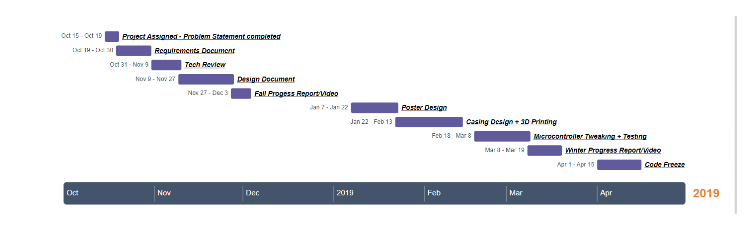
\includegraphics[width=1.0\textwidth]{GanttChartFinal.eps}

\begin{titlepage}
\vspace*{\fill}
\begin{center}

{\Large Tut-Tut, The IoT Rain Fall Detector Design Document}
\\[0.3cm]

{\large Team 21}
\\[0.3cm]

{\large CS 461 - Fall 2018}
\\[0.3cm]

{\large Michael Gillett, Casing and Microcontroller Lead}
\\[0.3cm]
{\large Jonathan Rohr, Data Collection and Management Lead}
\\[0.3cm]
{\large Shreyans Khunteta, UI Lead}
\\[0.3cm]

{\large November 26, 2018}
\\[1cm]

{\Large \textbf{Abstract}}
\end{center}
Tut-Tut, the IoT Raindrop Detector, is a project under the domain of the OPEnS (Openly Published Environment Sensing) Lab at Oregon State University. Tut-Tut will be able to detect a raindrop of any size, get an idea of the drop's mass from the intensity at which it falls, and detect the frequency of raindrops. After Tut-Tut gathers this data, it will be able to wirelessly transmit the information to a central server and communicate it to other IoT devices around Oregon State University. The detector will periodically wake up to check for rain and will stay awake as long as rain is detected within two minutes. If it does not detect raindrops within two minutes, it will go back to sleep. As a stretch goal, we will design an online mobile application to which the physical device will transmit information about the raindrops. If this stretch goal is not met, then the data will be stored in a Google Sheet.
\vspace*{\fill}

\end{titlepage}

\begin{center}
\section*{Glossary}
\end{center}

\quad \newline
\textbf{OPEnS Lab:} Openly Published Environmental Sensing Lab. Located at Oregon State University, this lab's goal is to develop environmental sensing devices and do research on their findings.
\newline
\newline
\textbf{CAD:} Computer-Aided Design. CAD is not a single program, but a technique used by many programs to design and simulate 3D objects that will be used in production.
\newline
\newline
\textbf{IDE:} Integrated Development Environment. Usually refers to the program being used to write and test the coded sections of the project.
\newline
\newline
\textbf{IoT:} Internet of Things. Used to describe a system made up of interconnected devices that form a network.
\newline
\newline
\textbf{Piezo Sensor:} Piezoelectric sensor. A device that uses the piezoelectric effect to measure changes in force by converting them to an electrical charge.
\newline
\newline
\textbf{MEMS Piezo Vibration Sensor:} Microelectromechanical systems sensor. Uses the piezoelectric effect to measure vibrations, but the sensor is small and its components are near microscopic.
\newline
\newline
\textbf{Accelerometer:} A device that measures vibrations from acceleration forces using electromechanical technology. It measures forces as voltages and then translates those voltages into vibration measurements.
\newline
\newline
\textbf{M0 Feather Microcontroller}: The M0 Feather is a microcontroller from Adafruit. It is thin, light and the centerpiece of our project. It will be handling all the computing for Tut-Tut.

\pagebreak

%\tableofcontents
\begin{center}
\begin{tabular}{ |p{0.3\linewidth}|p{0.3\linewidth}|p{0.3\linewidth}| }
\hline
\multicolumn{3}{|c|}{Design Document Revisions Table} \\
\hline
Section & Original & New \\
\hline
Overall &
Previously, this document consistently stated that Tut-Tut would be capable of measuring the specific mass of a raindrop. &
Now this document has changed all references to mass by replacing them with references to raindrop impact and intensity. Ultimately finding the specific mass of a raindrop was deemed out of scope for this project. \\
 & \\
2 &
The sensor will provide real-time information about the size/mass of the raindrops, how frequently they are falling and the intensity of the rainfall.. &
The sensor will provide real-time information about the relative size of raindrops when they impacts the sensor, how frequently they are falling, and the intensity of the rainfall. \\
 & \\
4.1 &
Using data gathered from the sensors, it will determine the size, density, mass, and frequency rate of these raindrops as they fall. &
Using data gathered from the sensors, it will determine the intensity of the rain based on the sensor impacts and the frequency rate of these raindrops as they fall.  \\
 & \\
4.1 &
These voltages can help determine the impact velocity and mass of the raindrops. &
Raindrops impacting the flat sensor will generate voltage that will be used to determine the intensity of the rain based on a specific range. \\
 & \\
\hline
\end{tabular}
\end{center}

\section{Design Document Introduction}
\subsection{Purpose}
This document will outline the design specifications referenced in each of the group members' Tech Reviews. We will discuss the design of the pieces, technologies, methods, and other parts that will be included in the final product. The final product may differ slightly from the specifications in this document, but it should act as a roadmap moving forward.

\subsection{Scope}
When the Tut-Tut reaches the end of its development, it will be expected to perform three major tasks and one task that will be implemented if there is time. First, it will need to be able to translate vibrations from rainfall into a voltage using its onboard vibration sensors. Second, it will transmit the collected data to the OPEnS Lab's Dropbox where it is subsequently stored into a spreadsheet in real-time. Third, it must be integrated into their existing ecosystem of sensors, Loom. Finally, if time permits, a browser UI will be used to communicate the Tut-Tut data in an easy to understand way.

\subsection{Document Overview}
First, Michael details the code we will use in our Microcontroller and describes the protective casing that will encase all components of our project. Second, Jonathan describes how we will be collecting rainfall data with sensors and how that data will be sent to our online database. Finally, Shreyans outlines what our stretch goal website would look like. The group members will be primarily responsible for all the technologies in their respective sections for the remaining time frame of the entire project.

\section{Design Document System Overview}
This product is designed to accommodate any person(s) who may want to know about rainfall metrics in their area. The sensor will provide real-time information about the voltage when the raindrop falls on the sensor, how frequently they are falling, and the intensity of the rainfall. These metrics could be used by meteorologist as a way to show more detailed information about the rain in the local area. They could also be used by farmers to better take care of their crop fields. Furthermore, the Tut-Tut Rainfall Detector will link into the OPEnS lab's larger ecosystem of environmental devices and sensors, known as Loom. The data Tut-Tut collects will be stored in a Google Sheets database for analysis.

\section{Design Document System Architecture}

\subsection{Code Design}
This section outlines the flow of the code flashed onto the microcontroller. 
\\
\\
We will be using an Adafruit Feather M0 microcontroller with Wi-Fi capability. The code that we will use can be divided into two phases: Initialization and Loop. The initialization section will set up all the necessary pins as soon as the device is booted, such as the LED and the analog pin used by the sensor. The looping portion of the code will run continuously, record the necessary data metrics, and upload them to the central server.
\\
\\
Once we test the sensor pieces and can record an accurate output of voltage (about a 1\% error), we will have an accurate threshold of voltage that will constitute a raindrop. In the main loop, we will first check the state of the sensor. If the voltage read is above our derived value, the program flow will enter an if-statement that will take care of the uploading. For good measure, we will have a delay function at the end of the loop to avoid overloading the buffer and losing our data.\cite{Knock} 

\subsection{Casing Design}
We have not yet done a model of Tut-Tut, but we do have a few expectations of what it should contain. First, we want the final product to be portable and able to be moved from place to place. To accomplish this we will need room in the casing for a battery, our microcontroller, and the sensor. Since the device will be out in rain, the casing containing the electronics will need to be weatherproof. The shape of Tut-Tut will likely be a 2 cm by 2 cm disk-shaped area on the top for raindrops to fall on, with a heavier base containing the hardware. Figure 1 shows what Tut-Tut might look like at the end of production given these specifications.
\newline

\begin{center}
Figure 1: A basic drawing of what Tut-Tut will resemble when complete
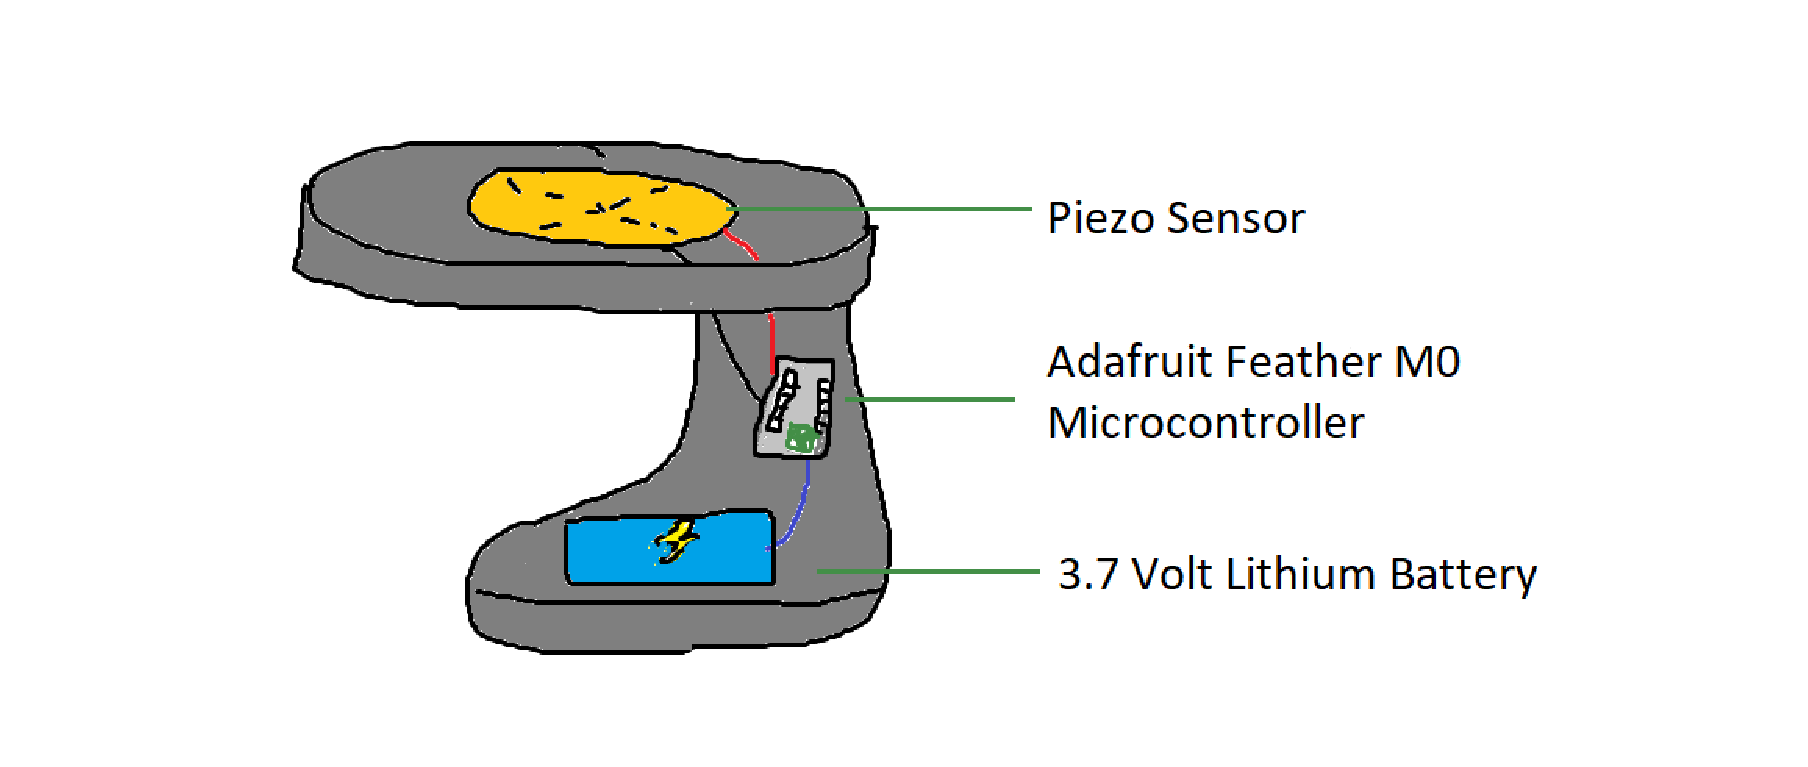
\includegraphics[width=.8\textwidth]{TutTutFirstDraft.eps}
\end{center}

\subsection{Design Rationale}
Each of the pieces of Tut-Tut had to be chosen specifically regarding the purpose of the final product. Trade-offs were (or will be) made on both the sensor and microcontroller pieces. For the microcontroller, we had the option of a basic board, one with Wi-Fi capability, and one with Long-Range Radio capability. We chose the Wi-Fi model because of the constant connection and reliable transfers of data. The sensors available to us are a piezo, a MEMS, and an accelerometer. These devices are all similar in usage and will only change the specific design of the 3D-printed casing depending on which is chosen.


\section{Design Document Data Design}

\subsection{Data Collection}
Tut-Tut will use sensors to register vibrations from raindrops. Using data gathered from the sensors, it will determine the voltage upon impact and frequency rate of these raindrops as they fall. We will be using the Piezo Vibration Sensor and the Piezo Element to accomplish these tasks. 
\\
\\
The Piezo Vibration Sensor is a MEMS sensor which uses the piezoelectric effect to detect vibrations. It has dimensions of around 1 cm wide and 2 cm long. It has a high voltage sensitivity of 1 V/g at its baseline and 6 V/g at its resonance. The sensor generates AC and voltage when the thin film gyrates. These voltages can help determine the voltage upon impact of the raindrops, which allows us to see where they fall within a certain range.
\\
\\
The Piezo Element is a basic sensor that also uses the piezoelectric effect to detect vibrations. Raindrops impacting the flat sensor will generate voltage that will be used to determine where the raindrop falls within a certain range. The two sensors perform the same task in different ways, so they each will be tested to determine which one will work best for Tut-Tut.

\subsection{Data Management}
Tut-Tut will be gathering data in the field. This means no one will be around to monitor its results immediately. All of the data that is collected by the sensors above will have to be sent wirelessly, in real-time, to an internet hub. We will use the PushingBox to Google Sheet Pipeline that has already been discovered by the OPEnSLab.\cite{pushingbox} As our Arduino Board gathers data from the sensors, it will make GET requests to a PushingBox Scenario using the data to be sent as URL arguments. The PushingBox Scenario formats the data and sends it as URL arguments in its own GET request to the Google Sheet. The Google Sheet will then parse through and display the data. PushingBox currently only supports 1000 requests per day per user. This means that Tut-Tut will only be able to send a string of data once every two minutes.

\section{Design Document Human Interface Design}
Currently our scope for the UI is limited. All the information and relevant performance metrics will appear as an Excel spreadsheet you can access through a website link. However, our stretch goal is to create a fully functioning user interface that the user can navigate. This fully functional user interface will be on a website that looks fairly similar to the OPEnS lab website (http://www.open-sensing.org/). 
\newline

\begin{center}
Figure 2: The current OPEnS Lab website. Tut-Tut's website will resemble this in aesthetic.\cite{OPEnSLab}
\includegraphics[width=.9\textwidth]{openslab.eps}
\end{center}

\subsection{Overview of User Interface}
This user interface will be built with programming languages such as HTML, CSS and JavaScript. The user interface design is still in progress and it is important to stress that this is a stretch goal. However, we want the final appearance of it to be visually appealing and engaging, and to be be usable and understandable by any educated user, and not just the OPEnS lab staff and students.

\subsection{Screen Images}
The images on the screen will be pictures of OPEnS staff and OPEnS lab projects, such as Tut-Tut itself. It will remain tasteful and aesthetically pleasing, and will incorporate Oregon State logos as well. We will have it try to remain the OPEnS lab webpages themselves.

\subsection{Screen Objects and Actions}
We may implement some minor transitions between pages to make the site look more appealing to the user. However we are not going to use JavaScript effects for the sake of JavaScript effects. We want every transition we do to be for the ultimate comfort and ease of the user. Our design for this will flesh out as the project goes forward, as this is still our stretch goal.

\pagebreak

\section{Design Document Conclusion}
This document will generally outline the remainder of Tut-Tut's production and give us a road map in which to reference as needed. First, the code will constantly loop checking for forces read from the Piezo above our calculated threshold, and take appropriate action when an exerted force does cross it. Next, we will have all of our hardware components contained in a waterproof casing that is bottom-heavy with a 2x2 cm disk-shaped surface area to measure the rain drops as they hit. The resulting voltages will be translated into meaningful data and sent through the PushingBox to Google Sheet Pipeline. Finally, if time permits, we will create a UI based off the OPEnS Lab website. It will be easily navigable by any user and will have performance metrics that Tut-Tut will be tracking (raindrop size, intensity and frequency rate). If we are unable to meet this stretch goal, the UI will simply be a Google Sheets document with all the relevant performance metrics.


\begin{titlepage}
\vspace*{\fill}
\begin{center}
{\Large Tut-Tut, The IoT Rain Fall Detector Tech Review}
\\[0.3cm]

{\large Team 21}
\\[0.3cm]

{\large CS 461 - Fall 2018}
\\[0.3cm]

{\large Jonathan Rohr, Data Collection and Management Lead}
\\[0.3cm]

{\large November 1, 2018}
\\[1cm]

{\Large Abstract}
\end{center}
Tut-Tut, the IoT Raindrop Detector, is a project under the domain of the OPEnS (Openly Published Environment Sensing) Lab at Oregon State University. Tut-Tut will be able to detect a drop of any size, get an idea of the raindrop mass from the intensity at which it falls, and detect the frequency of raindrops. After Tut-Tut gathers this data, it will be able to wirelessly transmit the information to a central server and store it in a database. This document will explore multiple possible technologies that can be used to gather, transmit, and store our data.
\vspace*{\fill}
\end{titlepage}

\section{Jonathan Tech Review Introduction}
Tut-Tut will be fully designed and 3D printed at the OPEnS lab. It will have a flat, circular sensor that can detect and measure minuscule hits and turn the Mechanical Energy produced into voltage for our microcontroller. The kinds of sensors that can achieve this are a piezo, a MEMS, or an accelerometer. These all have nearly the same functionality, but we will conduct tests on all 3 of them to see which fits our needs best. The flat sensor will be hooked up to a Feather m0 microcontroller that we will program using Artuino IDE. The microcontroller will be how we incorporate the readings and data manipulation we want, and also how we relay that information to the remote server. The data will be sent to the server using PushingBox API and will be stored in Google Sheets as it waits to be be parsed and analyzed. This document will review each type of sensor and explore alternate means of transmitting and storing the data.

\subsection{Collecting Data with a Sensor}
Tut-Tut will use a sensor to register the vibrations from raindrops. It will use the data from the sensor to determine the density, size, and speed of the rain drops. There are a variety of sensors that are capable of performing this task. Below are details on three types of sensors we will be physically testing before beginning our project so we can select the one most appropriate for our needs. The specific sensors that we end up using may be different from the ones referenced.

\begin{enumerate}
    \item \textbf{Grove - Piezo Vibration Sensor:} A piezoelectric sensor is any device that measures variables such as pressure, acceleration, and force using the piezoelectric effect. The sensor converts the forces it is subjected to into electrical charges which can be recorded and analyzed. \cite{piezosensor} For example, the Grove-Piezo Vibration Sensor offered by Seeedstudio can use the piezoelectric effect to measure vibration, impact, and touch. The sensor's sensitivity can be easily adjusted so we can gather precise data. It is lightweight, small, and thin which will help portability and aid in keeping Tut-Tut as small as possible. Their sensors have been used in car alarms, security systems, and low power wakeup switches. \cite{grovepiezosensor}
    \item \textbf{Accelerometer:} An accelerometer is a device that measures vibrations from acceleration forces using electromechanical technology. They measure the forces as voltage and then translate those voltages into a vibration measurement. \cite{accelerator} These measurements allow us to determine how fast the raindrops are as they impact the sensor, how much force is exerted on the sensor with each impact, and the frequency of the impacts. With this data we could figure out the density of the rain among other important factors. There are various types of accelerometers, including those that utilize the piezoelectric effect like the one above. Their are some that are meant to be as small as possible like the MEMS sensors described below.
    \item \textbf{Microelectromechanical Systems (MEMS) Accelerometer:} MEMS has to do with microscopic devices and systems. A MEMS accelerometer is an extremely tiny device that can perform all of the same sensing capabilities as an ordinary accelerometer. The accelerometers that utilize MEMS technology are usually the Capacitive type. They differ from their piezoelectric brothers by measuring the change of capacitance in the mass due to acceleration. MEMS allows these accelerometers to be cheaper and more compact. Unfortunately, most capacitive accelerometers suffer from a problem with high frequency noise due in part to their internal clocks and size. \cite{mems} This may not be an issue for our project, but it is important to keep in mind when analyzing our test data. 
\end{enumerate}

\subsection{Sending Data to an Internet Hub}
Tut-Tut will be gathering data in the field. This means no one will be around to monitor its results immediately. All of the data that is collected by the sensors above will have to be sent wirelessly, in real-time, to an internet hub. The best way to do this is by using the PushingBox API in the Arduino IDE. However, if that option didn't exist, there are two other possible ways of retrieving the data.

\begin{enumerate}
    \item \textbf{PushingBox API:} As stated above, the PushingBox API is the best way to send data to the internet hub in real-time. The main purpose of PushingBox is to instantly send notifications in various ways (emails, tweets, smartphone push notifications, HTTP requests, etc.) and can be called using Arduino. \cite{pushingbox} What we strive to do, however, is to push chunks of data in real-time to Google Sheets for storage. Luckily, the open-sensing team at Oregon State University has found a way to utilize PushingBox's real-time delivery of HTTP Ethernet data. We can use PushingBox API to transmit the HTTP data in a way that Google can recognize it as compliant HTTPS encrypted data. \cite{realtimepushingbox} With this system, we can continuously transmit data that Tut-Tut collects and store it directly into Google Sheets. Other data logging techniques require expensive secondary systems or creative solutions. This makes the PushingBox method the easiest and most effective way at transmitting our data from the device to the internet hub and directly into Google Sheets.
    \item \textbf{Omni Instruments Data Loggers:} If PushingBox wasn't available to us, then we may be forced to use other means of transmitting the data from Tut-Tut. One way is to hook it up to a GRD-3G Series Data Logger with Mobile and Satellite Communications which is offered by Omni Instruments. These devices are meant to be used to connect sensors to a communications network and transmit the found data to designated databases and/or web interfaces. The Data Logger is durable, reliable, and configurable. However, it suffers from bulkiness and excessive price. Depending on the features included, one device can cost between \$800 and \$1000. These devices are intended to be used for larger projects that transmit larger amounts of data than Tut-Tut and require a larger, near-global range. \cite{omni} 
    \item \textbf{SIM900A GSM Module:} If Tut-Tut was not able to connect to the internet hub because either it lacked the wireless adapter or it malfunctioned, a SIM900A GSM module could be used as a creative solution. Given the SIM900A has a working SIM card and is able to connect to the internet, it can be used to transmit data to a website or online database. Jens Christoffersen used a SIM900A GSM module to send temperature and humidity data to his website while he is was at the marina or at sea in his boat. He figured out a way to use a microcontroller, a SIM900A GSM module, various additional parts, and some PHP to transmit data from his sensors. \cite{jens} If this technology was to be applied to Tut-Tut, it would no longer need to have a constant connection to Wi-Fi. It could be placed in the middle of a forest and as long as it could connect to the cell towers, it would be able to still transmit data.
\end{enumerate}

\subsection{Storing and Managing Data}
All the sensor data that Tut-Tut will collect needs to be stored and managed somewhere. Preferably, it would be an online database of some kind so that multiple team members can view and analyze the data. It should also be organized and the GUI should be user friendly. 

\begin{enumerate}
    \item \textbf{Google Sheets:} The last section was focused on sending the data from Tut-Tut to the database. We saw that PushingBox API made it incredibly easy to store data directly into Google Sheets. This is accomplished through the use of clever scripts that the open-sensing team at Oregon State University has published online. The scripts allows Google Sheets to parse and display the data sent using PushingBox. Specifically, PushingBox sends formatted data as URL arguments for the GET requests it makes of the Google Sheet. \cite{realtimepushingbox} The project team can simply open up the Google Sheet and begin analyzing the data.
    \item \textbf{Microsoft Excel:} A Google Sheets alternative is Microsoft Excel or Excel Online. These options are not compatible with the PushingBox API method, so these would most likely be used if using an external data logger, such as the GRD-3G Series Data Logger. Excel is limited in its collaborative capabilities which makes analyzing data as a team difficult. Examples of people using Excel for data storage were also hard to find. One team used a mixture of complicated code and circuits to send a weather stations data directly to Excel. \cite{weather} Excel would not be a great option for Tut-Tut because not only is Google Sheets so convenient, but other alternatives like online databases would do the task with less complications.
    \item \textbf{MySQL Database:} MySQL is an online database management system that can be used to store all of Tut-Tut's sensor data. The data can be sent directly from the Arduino to the database with the use of PHP and Arduino code. \cite{mysql} MySQl is organized and has many management features that would aid in maintaining the database. Multiple team members can access and edit the database. MySQL, like Google Sheets, is also a free software/service which would help keep development costs low.
\end{enumerate}


\section{Jonathan Tech Review Conclusion}
Designing a large scale project requires tentative research before development can begin. This document is meant to outline the best choices available to us for each piece of the data collection and storage process. The product design specifications covered in this document will be designed according to the reviews given. We will test each of the three types of sensors specified and determine whether or not the Piezo Sensor, Basic Accelerometer, or MEMS Accelerometer are the best choice for our project. The most likely process of data transmission and storage will be the PushingBox to Google Sheets data logging. It is simple, easy, and provides true real-time data retrieval. This process of data collection to data transmission to data storage and management will be my responsibility until this project is completed.

\bibliography{myrefA}
\bibliographystyle{ieeetr}

\begin{titlepage}
\vspace*{\fill}
\begin{center}
{\Large Tut-Tut, The IoT Rain Fall Detector Tech Review}
\\[0.3cm]

{\large Team 21}
\\[0.3cm]

{\large CS 461 - Fall 2018}
\\[0.3cm]

{\large Shreyans Khunteta, Battery, IDE and UI Lead}
\\[0.3cm]

{\large November 1, 2018}
\\[1cm]

\begin{center}
    
{\Large Abstract}
\end{center}

Tut-Tut, the IoT Raindrop Detector, is a project under the domain of the OPEnS (Openly Published Environment Sensing) Lab at Oregon State University. Tut-Tut will be able to detect a drop of any size, get an idea of the raindrop mass from the intensity at which it falls, and detect the frequency of raindrops. After Tut-Tut gathers this data, it will be able to wirelessly transmit the information to a central server and store it in a database. This document will explore multiple possible technologies that can be used to gather, transmit, and store our data.
\vspace*{\fill}

\end{center}
\vspace*{\fill}
\end{titlepage}

\section{Shreyans Tech Review: Introduction}
Tut-Tut, the IoT rainfall detector is a project created and managed by the Openly Published Environmental Sensing (OPEnS) Lab located at Oregon State University. Tut-Tut will detect a raindrop of any size, gather it's mass based on the energy produced by the sensor, and measure the duration between the falling drops. All of the data gathered by Tut-Tut will be wirelessly transmitted to the OPEnS lab's central server and stored in an easily accessible spreadsheet. Tut-Tut should also be able to link up to the OPEnS lab's large ecosystem of wireless environmental sensing devices, known as Loom. Additionally, if time permits, we would like to have Tut-Tut's data be easily read by a browser UI application instead of buried in a spreadsheet.
\newline
\newline
This means that quite a few technical specifications have to be worked through. What languages will the UI be programmed in? What languages will the microcontroller be programmed in, and what IDE will we use to program it? What will the UI look like? What is the battery of the microcontroller that will power it? I hope to answer these technical questions in this document. However, to be upfront, this will be a much shorter tech review. There is simply just not as much to discuss with these pieces of technology.

\section{Shreyans Tech Review: The IDE}
\subsection{Arduino IDE}
In order to program the microcontroller, we need a place to actually write the code. For this, we will use the default Arduino IDE which can be downloaded for free from Arduino's website. An IDE is an integrated development environment, which means that it is used to maximise programmer productivity. It will point out compiler errors, have a source code editor, and so on.
\newline
The Ardunio IDE is a cross-platform IDE we will be using on our Mac and Windows machines. An Ardunio program (from here on referred to as a "sketch") is generally written in C or C++. The Arduino IDE allows us to compile a program and check it for correctness by using the "Verify" option at the top of the IDE. The right facing arrow allows you to upload a sketch to the microcontroller and actually "run" the sketch. \cite{Intel}  
\newline
In addition, the IDE will allow us to save our sketches and work on them later so we don't have to write them from scratch every time. If the user clicks on the magnifying glass icon, the Serial Monitor will open up. This is an exceptionally helpful tool during debugging. \cite{Intel2}
\newline
Without the IDE, there wouldn't be a project as this is the only thing that can upload the sketches we create to the Adafruit Feather M0.
\subsection{PlatformIO}
However, if you for some reason did want an alternative to the Arduino IDE, the most common one would be Platform IO. \cite{DZone} Not only can Platform IO support many Ardunio boards, it can also support Raspberry Pi. In addition, Platform IO is open-source and the source code can directly be downloaded from GitHub. The installation process is simple and straightforward. However, it has a library management system different from that of the Ardunio IDE, which can add some complications when the user simply wants to do a basic, easy task. \cite{FrancescoAzzola}
\subsection{Eclipse Ardunio IDE}
Eclipse is a very well-known integrated development environment which is largely used for Java development. However, with the right plug-ins, it can also be used for Ardunio development. The user can find this plug-in on the Eclipse marketplace. Once installed, the user has all the same features that they would be accustomed to with the Ardunio IDE, including serial monitors. It works just like a standard Eclipse IDE would, so there should be no difficulty in adjusting to the technology if the user is used to Eclipse. \cite{DZone}

\section{Shreyans Tech Review: The Battery}
There are two separate ways to power the Adafruit microcontroller. The user can first just simply connect the microcontroller to their laptop or desktop through a micro USB cable, and the Feather will regulate the 5V USB down to 3.3V. The user can also connect a 4.2/3.7V Lithium Polymer (Lipo/Lipoly) or Lithium Ion (LiIon) battery to the JST jack. The main use of the latter is to be able to take the Adafruit microcontroller on the go, but we'll likely be keeping it fairly close to our laptops for the time being. When we build the Tut-Tut IoT raindrop detector, we will use a 3.7V Lithium battery.
\newline
The dangers of using an improper battery could range from damaging the microcontroller circuits to starting a flame. Hence, selecting a correct battery is important. \cite{LadyAda}

\section{Shreyans Tech Review: The UI}
The UI exists in two states. We have a "stretch" goal of creating a fully functional website. If we do not meet this stretch goal, we will simply display an Excel spreadsheet that has all the data cleanly labelled and organized. We will be collecting data on performance metrics like raindrop size, raindrop intensity and frequency rate of rainfall. This Excel spreadsheet will be continually be updated by being connected to the IoT network.
\newline
However, if we DO meet our stretch goal, we will have a lot more functionality here. We will create a website using JavaScript, css and HTML. The page will look pleasing and will be associated with the OPEnS lab. It may possibly have an orange colour to better represent our university Oregon State. 
\newline
The UI will be easily navigatable. There will be ways to access specific bits of information (raindrop size, intensity and fall rate) and even do searches for specific days and rainfall statistics on those days. The CSS will be what we use for the styling, and we will use JavaScript on many of the transitions. However, this is strictly a stretch goal. We have so much work that will be spent in building this detector and making it capable of detecting raindrops that we may not be able to make this stretch goal work.
\newline
And now, to actually explain the technologies at work here...
\subsection{JavaScript}
JavaScript is a high-level, interpreted language, used by the vast majority of websites on the Internet. It was originally designed so that web browsers could be interactive, whether it be with moving images, or animations, or dozens of other possible interactive elements on a webpage. 
\cite{ChrisMinnick}
One of the biggest advantages of JavaScript is also that it is supported by ALL modern web browsers. So if we reach our stretch goal of creating a good mobile interface for Tut-Tut, we will be able to display that on Chrome, Firefox, Safari, Internet Explorer and all other browsers. Some browsers may not display JavaScript in exactly the same way but that's why the programmer must be diligent about writing correct code that works regardless of browser.
\cite{Wiki}
\subsection{CSS}
CSS, or Cascading Style Sheets, is a styling language. We use CSS in webpages to define the design and layout of that page. It also allows for the user to adjust for different screen sizes so that the webpage displays and looks good irregardless of which device it is being viewed on. \cite{W3Schools}

\subsection{HTML}
HTML, or Hyper Text Markup Language, is the structure of the Web. Webpages receive HTML files from webservers and render those files into webpages. Within HTML, scripting languages such as JavaScript can be embedded. We will extensively use HTML if we are able to design our website.
\cite{WikiHTML}

\section{Shreyans Tech Review: Conclusion}

Ultimately these three technologies - the IDE, the battery and the UI are crucial to our project. The IDE will help prevent us from making errors and to save our work. It will also be what we use to actually upload the sketches we create. The battery needs to be the correct type so that the microcontroller isn't damaged. The UI will be a stretch goal but one we hope to accomplish. We only have the option of really just one type of battery. We will likely use the default Ardunio IDE unless we come across a reason not to (which isn't the case yet) and we will extensively use JavaScript, CSS and HTML if we get to the point where we are creating a web application or website for Tut-Tut.

\bibliography{myrefC}
\bibliographystyle{ieeetr}

\begin{titlepage}
\vspace*{\fill}
\begin{center}
{\Large Tut-Tut, The IoT Rain Fall Detector Tech Review}
\\[0.3cm]

{\large Team 21}
\\[0.3cm]

{\large CS 461 - Fall 2018}
\\[0.3cm]

{\large Michael Gillett, Github and Microcontroller Lead}
\\[0.3cm]

{\large November 1, 2018}
\\[1cm]

\end{center}
\vspace*{\fill}
\end{titlepage}

\section{Michael Tech Review: Introduction}
Tut-Tut, the IoT rainfall detector is a project created and managed by the Openly Published Environmental Sensing (OPEnS) Lab located at Oregon State University. Tut-Tut will detect a raindrop of any size, gather it's mass based on the energy produced by the sensor, and measure the duration between the falling drops. All of the data gathered by Tut-Tut will be wirelessly transmitted to the OPEnS lab's central server and stored in an easily accessible spreadsheet. Tut-Tut should also be able to link up to the OPEnS lab's large ecosystem of wireless environmental sensing devices, known as Loom. Additionally, if time permits, we would like to have Tut-Tut's data be easily read by a browser UI application instead of buried in a spreadsheet.
\newline
\newline
A project such as this one will come with a caveat of decisions to be made. What should we design the model with? What language should the microcontroller be programmed in? What can we use to sense and read the rain that lands on it? These are not easy decisions, but with three of us and sufficient time to test we can narrow our options down significantly. Three key pieces of our device are the microcontroller board, the repository, and the casing that will house the sensor and microcontroller. 

\section{Michael Tech Review: Tech Review Pieces}
The three pieces that will be reviewed in this document. The other members of this group will review other pieces to be included in the device

\subsection{The Microcontroller}
The OPEnS lab at Oregon State University exclusively uses microcontrollers from Adafruit's Feather line of boards. Luckily for us, Adafruit makes several models intended for different project types. The three in focus are the Feather M0 basic, Feather M0 LoRa, and the Feather M0 Wi-Fi.
\newline
\newline
The Feather M0 Basic is the bare-bones model of the Feather family. It includes no additional features, but auxiliary capabilities can be added through soldering or wire hookup. This model of the Feather is very lightweight at 4.6 grams, and is about the size of a thumb. Despite being very light, hooking it up to a transmitter to send data to the OPEnS lab's server will significantly alter the portability of this product. Fortunately, they make models with transmitting capability, such as the LoRa Radio and Wi-Fi boards.
\cite{Basic}
\newline
\newline
The Feather M0 LoRa (long-range) Radio model specializes in communicating its information through transmissions up to 1 km. Unlike the Basic, this feature is embedded into the microcontroller. The data that can be transmitted must be small since the device uses a 900 MHz radio instead of ethernet or Wi-Fi. This is pretty negligible since Tut-Tut will not need to send heavy payloads, but it will need to be fast. The LoRa model also doesn't need the high power requirements of the Bluetooth or Wi-Fi models, but it is a little heavier than the Basic board at 5.8 grams.
\cite{LoRa}
\newline
\newline
The Feather M0 Wi-Fi model is just like it sounds. It is the Basic model, but with a Wi-Fi module added for high-speed and reliable data transfers. This allows for more complex data to be transferred, or for similar data (to the LoRa transmitting capability) to be sent very quickly. The Wi-Fi model requires more battery consumption than either of the previously mentioned boards, so we will need to consider how good our power source will be. Also, we will need to be within range of a Wi-Fi network. Adafruit's website states it is possible to make the board become its own access point, but that will require even more battery.
\cite{Wi-Fi}
\newline
\newline
Given these three boards available to us, the LoRa model seems to fit our needs the best. The Basic model is too barebones, and any additional features will need to be hooked up to auxiliary, and the Wi-Fi model will require too much battery consumption. 

\subsection{Github Repository}
All of our code is required to be posted in a repository under the domain of the OPEnS lab. How do we do version control on our project then? Thankfully we have plenty of software available to us.
\newline
\newline
Bitbucket is a version control application for Git projects and is very similar in every way. The difference is that the module for reviewing other members' code is a lot more robust. When you comment on someone's code, it creates a chain of replies underneath it, making it very easy to discuss the line(s) in question and make changes if necessary. The interface is also very seamless and integrates nicely into a team's server, and has full support for Jira issues and Trello cards. Bitbucket is also free for any team up to five members, making this a suitable choice for us if we need it.
\cite{bitbucket}
\newline
\newline
Another popular repository software we can make use of is SourceForge. SourceForge is dedicated to helping open source projects be as successful as possible. SourceForge's strength is that it allows for easy accessibility to other projects, which would make our project easier for other people to find. The website also highlights the most popular projects by week/month, allows for detailed download metrics, and has a very robust issue tracking system. Reviews of the site say there used to be glaring stability issues, but that they are now resolved. 
\cite{sourceforge}
\newline
\newline
Github has been the popular choice for open source projects for about 8 years now, and it doesn't appear to be going away anytime soon. Hosting the repository, making changes, and switching between versions are seamless and intuitive. Tut-Tut will be able to be tracked and well maintained on Github as well as any of these other sites. However, since the OPEnS lab's other projects are hosted on Github and we need to integrate Tut-Tut into their Loom network, it becomes the obvious choice in the situation. The three of us will have equal access to the main branch, as well as our own personal branches most likely, so we can test our own ideas and implement them in the main branch if needed.

\subsection{The Casing}
The casing will be 3D printed since it needs features and design specific to this project. In order to create the model, we will need to design it using a modelling program. There are a few pieces of software available to us, and this section will focus on AutoCAD, Inventor, and Onshape. 
\newline
\newline
Inventor is a 3D modelling software created by AutoDesk for product design. It offers high-level ability to generate shapes, set parameters, piece the shapes together into a model, and create accurate, detailed drawings. It also comes with collaboration support so your team can work simultaneously on your project. Inventor also supports non-native data, so if we were to base our Tut-Tut model off of one made in CAD, it would still be supported. The downside to this program is that it costs \$1,935 per year to use, which is just ludacris to spend on one project. Thankfully this is not our only option for modelling the casing.
\cite{inventor}
\newline
\newline
Another product design program available to use is Onshape. Onshape is like most other modelling programs, but offers its users cloud-based application support. This means no software updates, as well as easy accessibility to projects. Onshape also has a mobile application, so work can be done on the project from anywhere. The program itself is loaded with features that allow the user to create and model just about any product they can imagine. Just like Inventor, this product clocks in at about \$2000 per user per year. Given the fact that you can use it in any browser or on your phone, this program is a much more suitable choice over Inventor. However, there is still one more piece of software to look at: AutoCAD.
\cite{onshape}
\newline
\newline
AutoCAD is also from AutoDesk, and is the prized program for creating product models. It comes loaded with features for drawing 2D geometry and 3D models. AutoCAD goes beyond the other two in that the project can include specialized toolsets for the model type. This includes infrastructure, architecture in electronics, maps, and many more. Like the Onshape program, AutoCAD comes equipped with a mobile application that seamlessly integrates itself into the desktop version. AutoCAD also supports add-on apps or APIs included in the project. Surprisingly enough, it is the cheapest option out of the three at \$1500, and appears to be the most friendly to beginners.
\cite{autocad}
\newline
\newline
Given these choices, the definitive program we will use is AutoCAD. The three of us have never designed a product using CAD before, and the OPEnS lab already has it installed on their computers, meaning that we wouldn't have to shell out 1500 dollars just to design one product. 

\section{Michael Tech Review: Conclusion}
Designing a large scale project is no easy task: there will be many choices made along the way. This document is meant to give us an outline so that important decisions are made ahead of time or with an informed background. The product design specifications covered in this document will be designed according to the reviews given. The microcontroller will be either the Long Range Radio or Wi-Fi models, since they are very similar and can be switched out pretty easily. The repository will definitively be Github for ease of access and Loom compatibility. Finally, the CAD program we will use to design this product will be AutoCAD due to availability and user-friendliness. These pieces of Tut-Tut will now be my responsibility to overview and maintain throughout the project timeline.

\bibliography{myrefB}
\bibliographystyle{ieeetr}

\pagebreak

\section{Jonathan’s Weekly Progress}

\section{FALL 2018}
\subsection{Week 4}
This week, my group and I met up in the library and the OpensLab on two separate occasions to try and figure out how to connect our Adafruit microcontroller to our computers. Unfortunately we could not figure it out because it turns out it was a faulty one. We got a new one that works perfectly and successfully made the LED on it blink steadily. Personally, I got to meet our client Chet face to face for the first time. Our plan is to get together with Chet next week to discuss what is next for us. I still need to print off and sign a saftey waiver before I can use equipment in the OpensLab.

\subsection{Week 5}
This week, my group and I contacted our client to discuss the requirements for our project. He presented us an organized list of most specifications for our project and we started to work on the requirements document Friday. We didn't get to meet up at all this week due to midterms, but we were able to chat online while working to ensure we were all on the same page. Next week, we plan to finish up the requirements document and start on our individual tech review assignments.
\subsection{Week 6}
This week, my group and I completed the requirements document and our individual tech reviews. We didn't get to meet up at all this week due to midterms, but we texted to coordinate what pieces of the project each of us was going to review. Next week, we plan to meet up with the client to learn what our weekly task will be and we will discuss the tech review final draft. We will make sure we are on the same page as the client in our meeting when we show him our requirements document.
\subsection{Week 7}
This week, my group and I completed our individual tech review final drafts.  One member of our group met with the client on Thursday and received new plans for the coming week. Our client wants to test 3 different vibrations sensors. We will use our microcontroller to prove that each sensor can detect vibrations and show him. We had no problems this week, although we weren't able to meet up to talk about the tasks during the weekdays. My group and I plan to meet on Saturday to discuss the Thursday meeting more and start working on the tasks our client gave us.
 
\subsection{Week 8}
This week, my group and I ordered a piezo sensor and a mems sensor so that we can test them in the coming weeks.  I met with the client on Thursday and received new plans for the coming week as well as solidifying our end of term goals. Our client wants us to test 3 different vibrations sensors once we receive them. He also want us to explore different apparatuses that can be used to distribute "rain drops" of specific masses. We had no problems this week, although we weren't able to meet up to talk about the tasks during the weekdays. My group and I plan to meet on Saturday to discuss the Thursday meeting more and start working on the tasks our client gave us.

\subsection{Week 9}
This week, my group started working on the design document and planned on testing the sensors that our client wanted us to test. Unfortunately, one of our group members was in a car accident so he was stranded in Beaverton for the week. We were unable to test the sensors because he was the one who had ordered them. Once he gets back in town, we will be able to test the sensors and deliver the results to the client.
 
\section{WINTER 2019}
\subsection{Week 1}
This week, my team met on Wednesday to plan out the next two weeks. We listed the top tasks we needed to complete in that span. We met on Friday to test the Piezo and MEMs sensors. Next week, we will start designing our 3D printed base in the OPEnS lab. We plan on setting up a meeting with our client as soon as possible so that we can touch base.
\subsection{Week 2}
This week, my team met on Thursday to meet with our client. However, our client did not show up. Instead we sent him an email with our progress. We will meet on Friday to test the mems sensor and on Monday of next week to start designing the casing.
\subsection{Week 3}
This week, my team met on Thursday to meet with our client and discussed our plan for the next couple of weeks. We will be testing each of the three sensors to determine which one is the most viable for sensing rain drops. We will perform these tests by dripping water on a sensing platform and measuring the sensitivity. My group met Friday to start our tests with the piezo and MEMs sensors. Next week, we will try and test the accelerometer and also order some materials we will need.
\subsection{Week 4}
This week, my team met on Wednesday and ordered some supplies through the OPEnS Lab. We planned to start learning AutoCad in order to design parts of our product that need to be 3D printed. This weekend, we will individually teach ourselves through tutorials so we can start printing next week. We can't do any testing of the sensors without our supplies that we ordered so we will be focusing on the AutoCad stuff until the supplies arrives. 
\subsection{Week 5}
This week, my team met on Monday and Wednesday to test our sensors in the OPEnS Lab. We are going to meet on Sunday to design parts of our product that need to be 3D printed. On Thursday, our group met with another group to critique each others posters. We got some insight of how to better format our information and draw the viewer into our project. 
\subsection{Week 6}
This week, Shrey and Michael designed some prototype sensing area in Fusion 360 and we plan on getting them 3D printed on Monday. I worked on code that would allow us to record the average amplitude of the rain drops over a period of time. This will allow us to visualize if the intensity of the rain is light or heavy. I will be working over the weekend to set up a internal timer that will aid with the intensity while also allowing us to determine frequency of the rain drops. We could also use a similar timer to determine duration of a rain. I will also need to research how to put the board to sleep when there is no rain and have it wake up at the first drop.
\subsection{Week 7}
This week, Shrey and Michael designed some additional prototype sensing area in Fusion 360 and we 3D printed them during the week. We now have 3 prototype sensing area that I will be using for our testing. I will be working over the weekend to set up a internal timer that will aid with the intensity while also allowing us to determine frequency of the rain drops. We could also use a similar timer to determine duration of a rain. I will also need to research how to put the board to sleep when there is no rain and have it wake up at the first drop.
 
\subsection{Week 8}
This week, Michael began work on designing the 3D printed enclosure for the electrical components of our project. I will work this weekend to implement the Pushing Box API code into our code so that the data is sent to Google Sheets. We didn't get to meet much this week, unfortunately, but most we have to do can be done individually. We plan on having the enclosure printed by next week and the code complete. We will then be able to start our final testing phase.

\subsection{Week 9}

This week, Michael 3D printed enclosure for the electrical components of our project. I will work this weekend to implement the Pushing Box API code into our code so that the data is sent to Google Sheets. We plan on testing the prototype next week and have the code complete and bug tested.

\subsection{Week 10}
This week, Michael 3D printed another enclosure for the electrical components of our project. This one is slightly larger since our other one did not fit the breadboard we are using. This one fits all of our components perfectly. I will work this weekend to implement the Pushing Box API code into our code so that the data is sent to Google Sheets. I will also test the prototype this weekend. We met on Thursday to film most of our video progress report. We will finish it up this weekend and turn it in on Tuesday.

\section{SPRING 2019}

\subsection{Week 1}
This week, my group and I discussed the poster and final 3D printed casing. We gave each other tasks to complete by next week. I finished fixing bugs with our code that wasn't putting the board to sleep. It now sleeps for a certain amount of time, checks to see if it is currently raining, then goes to sleep again if it is not. This repeats until it is raining, at which time it runs our data collection code. We plan on doing some last minute testing before the code freeze and will be done by next weekend.
 
 
\subsection{Week 2}
This week, my group and I discussed the poster and final 3D printed casing. We plan on doing some last minute testing before the code freeze and will be done by this weekend. After the code freeze, we will get our final casing printed and our poster done. 
\subsection{Week 3}

My team and I designed and printed our final casing on the better 3D printer in the OPEnS Lab. We have begun final tests to fine tune our code. We edited our documents to reflect the small changes we made. We plan on meeting Sunday to make our poster board.

\subsection{Week 4}

My team and I designed and printed our final casing on the better 3D printer in the OPEnS Lab. We completed the poster board on Monday and got it reviewed by our client. We will be doing some final tests next week. 

\subsection{Week 5}

My team and I have had trouble meeting with our client to demo our project because he is so busy. We hope to demo it for him this week so we can show him all we have done. We also need to ask him about weather proofing our casing further.

\subsection{Week 6}

My team and I gave our client a demo on Wednesday. He gave us some suggestions and also gave us a list of documentation we need to get ready before the project hand off. We are going to work this weekend on implementing his suggestions and typing up test procedures. We will also create a state diagram for our code.
\pagebreak

\section{Michael’s weekly progress}

\section{Fall 2018}

\subsection{Week 4:}

This week we worked on setting up our microcontroller and working with the Arduino IDE. We each spent about an hour trying to get our computers to recognize the device, and upon returning to the OPEnS lab, found out it was the fault of the microcontroller itself. We got a new one and it worked flawlessly, and we programmed it to blink its LED.
Plans for the future are to do more advanced operations using the Arduino IDE and consulting the lab staff about peripherals we might need, like an antenna or a battery.

\subsection{Week 5:}

(No submission)

\subsection{Week 6:}

Progress
This week we made our requirements document and tech review which gives us a more concrete, realistic timeline for our project. I feel much better now that it's all down on paper and I know where we should be at a given point of time, as well as knowing all of the technology we will be using to build the project.
\newline
Problems
No major problems were encountered, but we did feel a little bit repetitive when we were writing the requirements document. We collectively decided that it was better to keep it concise instead of being too wordy. For the Tech Review, we found it difficult to come up with 9 different pieces of the project that we could do in-depth research on. We eventually reached a basis, and the final result is one we're happy with.
\newline
Plans
We plan to write our design document and progress report in the coming weeks. On Sunday, we will meet and try to learn about CAD design so we can get a head start on designing our product.
\subsection{Week 7:}
Progress
This week, in our client meeting, Chet clarified that our Tech Review is extremely important and will be the basis of our grade for this term.  He also assigned us new tasks for testing pieces that will read vibrations from landing raindrops. A piezo, a MEMS, and an accelerometer are what he wants us to test
\newline
Problems
No problems this week
\newline
Plans
This weekend, we plan to meet up and try to get an idea of what our product will look like when it's done. What we want our CAD model to be, essentially. Also, we will look at the upcoming assignments.
 
\subsection{Week 8:}
Progress
This week we ordered the sensors we will need to conduct the energy from the falling rain. These sensors will be wired to the microcontroller and included in the casing
\newline
Problems
No problems this week
\newline
Plans
We will wire the sensors to the board, and try to test that the sensors accurately measure synthetic drops of rain. Then we will start designing the dimensions of the casing that will hold all the hardware and essentially be Tut-Tut itself.
 
 
\subsection{Week 9:}
Progress
The parts we ordered have arrived and we can begin work on our testing. We ordered several devices to measure energy in the form of voltage, which we can read using the microcontroller.
\newline
Plans
We will hook up these measurement devices (MEMS, Accelerometer, and Piezo) and test them using droplets of water acting as rain drops.
\newline
Problems
Unable to check mail as a car crash has a left me stranded in Beaverton, away from my mailbox. But I trust that they arrived safely. No other problems this week.
 
\section{Winter 2019}
\subsection{Week 1:}
Progress
We made no progress over winter break
\newline
Problems
We couldn't meet up because we were all in different cities
\newline
Plans
Get to work designing Tut-Tut's casing in CAD software
 
\subsection{Week 2:}
Progress
This week, we tested our piezoelectric sensor at the OPEnS lab and got an idea of how to set up our circuit to read rainfall intensity, and scheduled our weekly meetings with our client.
\newline
Problems
Figuring out the circuit was somewhat difficult, and we don't know how to test the third kind of sensor that our client wants us to test before prototyping. 
\newline
Plans
Meet at the OPEnS lab every MWF from now on, and meet with Chet on Thursdays. The next step is to design the casing for our product in AutoCAD and printing it at the OPEnS lab.
 
\subsection{Week 3:}
Progress
This week we made progress by testing out our three types of sensors. Jonathan and I tested the piezoelectric and MEMS sensors, and Jonathan and Shrey tested the accelerometer. We found that the MEMS was more sensitive, but only gathered readings when a small gold part was touched. Anything in proximity didn't set the MEMS off, but hitting the table next to the piezo did. I don't know about the accelerometer testing, but we will likely go with the MEMS on this one.
\newline
Problems
Every time we set up Arduino IDE, we have trouble connecting the microcontroller to the computer. The first time it was our board, but this most recent time it was the cable we used to connect it. We have to be a lot more careful about choosing cables that will consistently work how we expect. Another problem is that I'm really busy with other homework and had to cancel on meeting up with them. As the term goes on it will be harder and harder to juggle all the coursework.
\newline
Plans
Once we test all the sensor types and come up with a verdict, we will begin designing the casing that will essentially be our product itself. It will hold all the essentials inside (microcontroller, wires, battery, breadboard if needed) and should be waterproof. We will use AutoCAD to design it and it will be 3D printed at the OPEnS lab.
 
 
\subsection{Week 4:}
Progress
This week, we set up testing methods for raindrops on the sensors, which we will use to test how accurate they are. We worked with an OPEnS lab member, Gray, to get help setting up the testing station and for providing an accelerometer. Progress was limited because all members were sick.
\newline
Problems
As always, we had problems setting up Arduino IDE to recognize our microcontroller. It seems to be tied to the kind of cable we use to connect it. We also had problems setting up the rig we will use to test using pipettes, but it all worked out after some time.
\newline
Plans
Next week we will test the sensor's accuracy using the rig and record our findings. We will also begin working with AutoCAD to design the casing which will house our electronic components.
 
\subsection{Week 5:}
Progress
This week we thoroughly tested the MEMS sensor and Piezo sensor using a homemade rig to drop water on the sensor plate from 1 meter above using pipettes. The results found were very telling.
\newline
Problems
The main problem we have now is that the readings from the sensor are displayed as a voltage between 0 and 5 volts. We need a way to convert the voltage into a value of force so it will have more meaning at a glance.
\newline
Plans
On Sunday, we will meet and attempt to design our casing, or at least the disc shapes we want to test and get them ready for 3D printing at OPEnS Lab. We will also do research on our own to find out how to convert voltage readings into measures of force/impact.
 
\subsection{Week 6:}
Progress
We designed the Disk shapes we need using Fusion 360 software and scheduled a time to 3D print those models, we will use them with our raindrop tester to gain metrics on which one records data the best.
\newline
Problems
We originally tried to design these parts in AutoCAD which was extremely frustrating, but Fusion 360 was recommended to us in place of it and it has been infinitely better for us.
\newline
Plans
We will print those disks to test and then get started on developing the full model of our product.
 
\subsection{Week 7:}
Progress
This week we printed off more designs for our detection area. We also decided we should print one model with a slanted disk area to avoid water collection as best we can.
\newline
Problems
We ran out of printing material during the second set of disks so we could not test them. The good news is that the ones we did print are much more viable and realistic to be used in the final product. Also, our initial disks were too thick to record any vibrations, so we had to make them much thinner.
\newline
Plans
This weekend we will do our progress report, and work on designing the casing which will be our beta.
 
\subsection{Week 8:}
Progress
We finished and turned in our progress report rough draft and have conducted our peer reviews.
\newline
Problems
No problems were encountered
\newline
Plans
We will finish designing and printing our prototype model that will be displayed at expo this upcoming week
 
\subsection{Week 9:}
Progress
The prototype pieces were successfully printed. All that is left is to put the pieces together with all the electronic components inside. 
\newline
Problems
The first time I tried to print, it failed because the spool got caught on itself during the second layer. I stayed for 15 minutes into the print and it seemed fine so I left only to discover the next day that it had failed.
\newline
Plans
Put the pieces together and have Jonathan figure out the PushingBox API
 
\subsection{Week 10:}
Progress
We got our prototype pieces printed and made sure all of the electrical components fit inside, and dropped a few simulated raindrops onto it to make sure it would hold up like we thought
\newline 
Problems
No problems this week
\newline
Plans
We plan to finish the PushingBox API over the weekend and then when that is configured we will print a refined, final prototype using the OPEnS lab's highest quality 3D printer
 
\section{Spring 2019}
\subsection{Week 1:}
Progress 
Jonathan figured out the sleep function for our device. We should be good for the Code Freeze.
\newline
Problems
None so far but we may encounter one when we try to design the new 3D printed casing.
\newline
Plans
Print out a final prototype for our casing using Fusion360. We will then waterproof it and attempt to test our device in a real outdoor environment

\subsection{Week 2:}
Progress
We have not done much this week besides Jonathan figuring out the sleep mechanism for our code. We should be good for the code freeze next week.
\newline
Problems
No problems this week
\newline
Plans
Finish designing the casing, update our documents and poster, and send them to our client for verification.
 
\subsection{Week 3:}
Progress
We updated our documents and had our client verify them. I worked on our casing a little more too.
\newline
Problems
We had a few troubles with the makefile when compiling our updated documents but figured then out.
\newline
Plans
Work on our poster and print the new casing
 
\subsection{Week 4:}
Progress
We finished our poster and 3D printed the casing we will use to hold our electrical components.
\newline
Problems
The base of the casing didn't print right the first time, but it was an easy fix and didn't take long to print a new one.
\newline
Plans
No real plans as of right now besides demoing our device to our client. Will standby for further instruction.
 
\subsection{Week 5:}
Progress
No progress this week, aside from submitting our poster. Progress from this point on will be very minute in comparison to the previous reports since we are in the final stretch.
\newline 
Problems
We are having a hard time meeting up with our client due to his busy schedule
\newline
Plans
Unsure about plans from this point besides preparing for expo. Will await instructions from Kirsten or TAs.
 
\subsection{Week 6:}
Progress
This week we demoed our project to our client, and he gave us praise and constructive criticism. I think it went really well and he is happy with our work this term
\newline
Problems
We had to change a few calculations to better reflect the rain intensity, and we had failed to catch a potential divide-by-zero error as well. We caught and fixed them before any major problems occured.
\newline
Plans
Get our final checklist items completed, and attend expo! We are going to create a state diagram for our product and write thorough procedures and documentation


\pagebreak

\section{Shreyans Weekly Progress}

\section{Fall Term}
\subsection{Week Four}

Progress: This week we acquired our Adafruit Feather from the OPEnS lab. At first none of us could make it work. We tried everything across a variety of devices. Turns out we had gotten a broken microcontroller. We got a working one, and got the LED to blink.
\newline
Problems: The fact we started with a broken microcontroller.
\newline
Plans: Working with Chet to set up a regular meeting time.


\subsection{Week Five}

Progress: Got a full set of project requirements from Chet. Setting up a regular meeting time to start designing the detector. Set up a regular meeting time with Chet at Thursdays at 10.
\newline
Problems: It's pretty apparent Chet's going to be busy. But that scheduled meeting time should help.
\newline
Plans: We're going to be starting to really get our hands dirty and learning the new technologies we'll need to know to build the detector

\subsection{Week Six}

Progress: Finished Requirements. Finished Standards.
\newline
Problems: Couldn't meet with Chet this Thursday. He just didn't show up. Not a single group was able to meet with him.
\newline
Plans: To finish Tech Review and hopefully meet with Chet.

\subsection{Week Seven} 

Progress: Met with Chet and he gave us some other, further goals. Finished Tech Review.
\newline
Problems: N/A this time.
\newline
Plans: To finish the tasks Chet assigned.

\subsection{Week Eight}

Progress: Met again with Chet, ordered supplies/equipment we needed.
\newline
Problems: It was mostly a holiday week - we had Monday off and everyone got busy with holiday plans.
\newline
Plans: Meeting tomorrow to start implementation.

\subsection{Week Nine}

Progress: Not much. Started a bit on Design Documents.
\newline
problems: Michael’s car got totalled so he can’t access his mailbox and get the sensors.
\newline
plans: Busy next week when we really start building this bad boy.

\section{Winter Term}

\subsection{Week One} 

Progress: I attended school.
\newline
plans: Work on furthering project
\newline
Problems: Forgot to do this report for some time.

\subsection{Week Two}

Progress: Met with team, finished some BaseCamp tasks, sent relevant emails.
\newline
Problems: Professor Udell couldn’t make it to our scheduled meeting.
\newline
plans: Finish accelerometer work.

\subsection{Week Three}

Progress: Met in OPEnS with Chet, built a basic prototype and chose our sensors.
\newline
Problems: Figuring out how to work with the intensity of rainfall - also, I got very sick.
\newline
Plans: Further work on the sensor.

\subsection{Week Four}

Problems: N/A
\newline
Progress: Started learning how to use AutoCAD.
\newline
Plans: Further work on building the detector.

\subsection{Week Five}

Progress: We worked more on building our project, and met with Kristen about our poster during poster review. Met with TA.
\newline
Problems: Forgot to do this review again. Going to start setting up reminders on my phone or just doing it Thursday nights.
\newline
Plans: To do this review at the right time this week, finish the AutoCAD design of the dome.

\subsection{Week Six}

Progress: A LOT actually. We figured out how to calculate the average voltage, AND we found out a software called Fusion360 is much better than AutoCAD for 3D modelling. So we've now created quite a few domes and disks and just gotta print them. Things are looking up.
Plans: Finish the printing, get it attached, and figure out Internet connectivity.
Problems: Class and work. Those two things interfere with the project.

\subsection{Week Seven}

Progress: A lot. Finished our 3D prints.
\newline
Plans: Do progress report, Internet connectivity.
\newline
problems: Other classes, job

\subsection{Week Eight}

Progress: Finished and submitted progress report and reviewed another group's.
\newline
Problems: N/A
\newline
Plans: Finishing the project.

\subsection{Week Nine}

Progress: More work on the casing/code of the project.
\newline
problems: Just time.
 \newline
plans: Finishing project, shooting video.

\subsection{Week Ten}

Progress: Worked on the casing for Tut-Tut, recorded video.
\newline
Plans: Finish anything else that needs to be done to get project to Alpha.
\newline
Problems: Dead week, finals week.

\section{Spring Term}

Problems: Everyone got sick. None of us could make it to the week one senior design meeting at 8 am.
\newline
Progress: Continued testing on our project, going to do the final prototype print, we are well on our way.
\newline
Other: N/A

\subsection{Week Two}

Progress: updated documentation, met with TA
\newline 
Problems: N/A
\newline 
plans: finish documentation, finish poster board, get reviewed by Chet 


\subsection{Week Three}

Progress: Gave Chet documents for client verification, attended a faculty lecture.
\newline
Problems: N/A
\newline
Plans: Working on the final poster.

\subsection{Week Four}

Progress: We finished our poster board and had it reviewed by client.
\newline
Plans: Doing a live demo for our client and the instructors.Printing the board.
\newline
Problems: N/A

\subsection{Week Five}

Progress: Finished and submitted poster. Went to speaker session on 5/3.
\newline 
Plans: getting poster print, prepping for expo
\newline 
problems: Chet hasn’t responded to when he wants to see a live demo 

\subsection{Week Six}

Progress: attended the lecture in class, demo'd project to Chet
\newline
Plans: Expo next week!
\newline
Problems: N/A
\newline

\section{Poster}
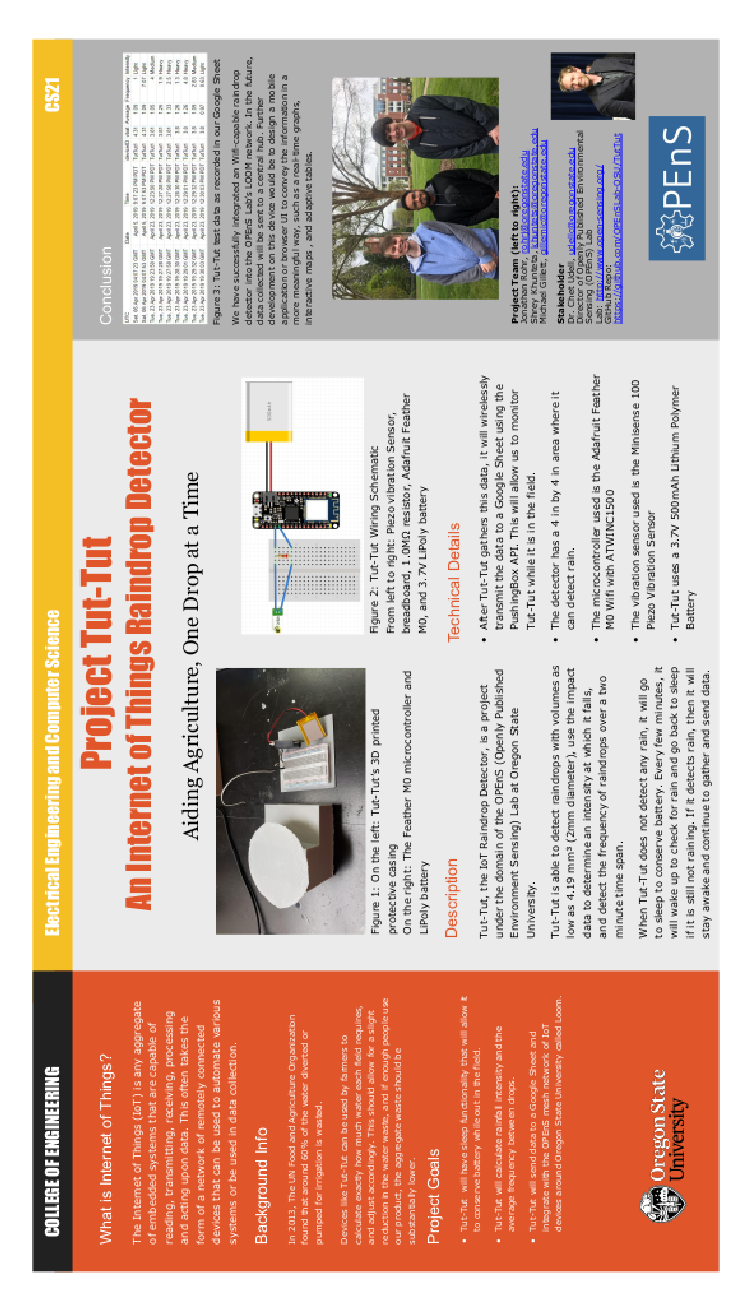
\includegraphics[width=0.7\textwidth]{TutTut_Poster.eps}

\section{Project Documentation}
\subsection{How Tut-Tut Works}
Tut-Tut, when powered on, will begin polling for 20 seconds. If a raindrop is detected within those 20 seconds, it will start data collection. If not, it will go to sleep for 2 minutes before polling again. In the data collection mode, it will collect all raindrops that were recorded over the course of 1 minute, average them, and upload those values to our spreadsheet. When no values are recorded, it will upload "Rain Free" to the spreadsheet and go back to sleep.
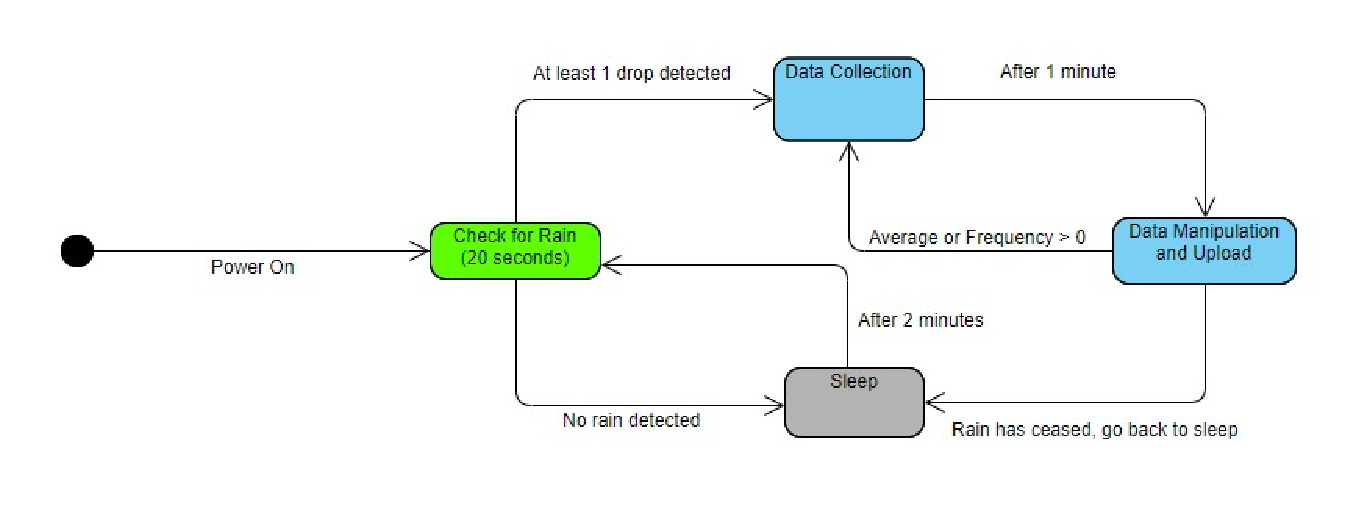
\includegraphics[width=1.0\textwidth]{TutTut_FSM.eps}

\subsection{How to Install Software and Run Tut-Tut}
First, you should have already downloaded the Github repository, located at https://github.com/OPEnSLab-OSU/TutTut
\newline
\newline
Step 1: Navigate to https://www.arduino.cc/en/Main/Software and select the appropriate download based on your operating system.
\newline
Step 2: Install the latest Arduino IDE version.
\newline
\newline
Remaining steps based on Windows version
\newline
\newline
Step 3: By default, the installation will place an Arduino folder in the Documents System Folder. Other destinations can be specified during the installation.
\newline
Step 4: Move the libraries and piezo\_vibration\_sensor folders from the TutTut\_Code folder of this repository into the Arduino folder at your specified destination.
\newline
Step 5: Move into the piezo\_vibration\_sensor folder and open the piezo\_vibration\_sensor.ino file. This will launch the Arduino IDE.
\newline
Step 6: Additionally, open up the config.h file and navigate to the Wi-Fi SETTINGS section. Change the DEFAULT\_NETWORK and DEFAULT\_PASSWORD to the desired network and password.
\newline
Step 7: Connect the TutTut device to your computer via a microUSB cable.
\newline
Step 8: In the Arduino IDE, click the Tools dropdown menu at the top.
\newline
Step 9: Where it says Board: "XXXXX", select Adafruit Feather M0 from the additional dropdown menu.
\newline
Step 10: Now press the upload button (Right Arrow) to compile and upload the sketch to the microcontroller in the Tut-Tut Device.
\newline
Step 11: The code should start immediately after the upload is complete and will continue to run unless disconnected from power. The USB can now be disconnected and the battery can be connected.
\newline
\newline
\newline
Tut-Tut Installation Guide Command Line On Linux
\newline
\newline
Step 1: Go to Arduino site and follow the necessary steps listed: https://www.arduino.cc/en/guide/linux
\newline
Step 2: Once installed, follow similar steps to the above to upload the sketch to the microcontroller.
\newline
\newline
Setting up the Google Sheet
\newline
\newline
Follow this guide: https://github.com/OPEnSLab-OSU/InternetOfAg/tree/master/PushingBox

Add all configurations mentioned in the guide into the config file in the piezo\_vibration\_sensor folder.

\subsection{Hardware Needed}
Adafruit Feather M0 Wi-Fi Microcontroller with ATWINC1500
\newline
AUCH Disposable Plastic Pipettes: 2mm, 3mm, 4mm
\newline
Large Dropper: 2mm
\newline
TAZ LulzBot 3D Printer
\newline
Breadboard
\newline
1.0MΩ Resistor
\newline
3.7V 500mAh Lithium Polymer Battery
\newline
Minisense 100 Piezo Vibration Sensor
\newline
\newline
The .f3d and .stl files contained in the TutTut Github repository are the design for the casing, and must be 3D printed according to the specifications. Does not have to be printed from a TAZ Lulzbot 3D Printer.
\newline

\subsection{Wiring Guide}
The negative pin of the Piezo sensor needs to be connected to GND on the microcontroller. The positive pin of the sensor needs to be connected to A0 on the microcontroller.
\newline
\includegraphics[width=1.0\textwidth]{wire_guide.eps}

\subsection{Testing Procedure}
\begin{enumerate}
    \item Open up piezo\_vibration\_sensor.ino in the Arduino IDE
    \item Upload sketch to the microcontroller from the Arduino IDE
    \item Make sure Tut-Tut is connected to a charged battery or a computer
    \item The device will turn on the moment it is provided power
    \item Place Tut-Tut on a stable surface
    \item Open up the Google Sheets that the PushingBox API is sending information to
    \item Fill up pipette with water
    \item When Tut-Tut turns on, start dropping drops on the surface, which should be recorded on the Google Sheets
    \item Use different pipettes with varying drop sizes to simulate different rain drops.
\end{enumerate}

\subsection{Suggestions for Improvement}
\begin{enumerate}
    \item If Tut-Tut was used in the field, the battery would not last very long in a rain storm. We suggest coming up with other ways to power Tut-Tut or figure out how to ensure Tut-Tut can operate at extremely low power mode. It has a sleep function for when it isn't raining (which can also be improved), but it drains too much power during constant use.
    \item We had a farmer suggest that Tut-Tut should not only be able to provide info to the farmers themselves, but also have the ability to communicate with pivots out in the fields. Tut-Tut could calculate how much water has fallen based on the frequency and intensity and would either activate the pivots or keep them idle. This may be out of scope, but it is an interesting possibility to think about.
\end{enumerate}

\section{Recommended Technical Resources}
http://www.open-sensing.org/\#intro
\newline
http://www.open-sensing.org/resources
\newline
https://github.com/OPEnSLab-OSU
\newline
https://www.arduino.cc/en/Main/Software
\newline
https://www.autodesk.com/products/fusion-360/students-teachers-educators
\newline
\newline
Some people who were incredibly helpful were the staff in the OPEnS Lab. Chet Udell was invaluable, as were people like Garen Porter who aided us in learning how to manage Fusion360 and 3D printing as a whole.

\section{Reflections}
\subsection{Shrey's Reflection}
I learnt a lot more about Arduino, IoT and 3D printing in particular. One of the reasons I wanted to do this project was to pick up new skills that were more hardware inclined. I’m a Human-Computer Interaction applied option here at OSU, and my minors are in Psychology and Writing. While I love my unique background, I wanted a more technically focused project that would allow me to show off some newly gained skills. And this worked! I especially became very proficient with 3D printing and Fusion360, and I learnt a lot of tools I otherwise wouldn’t have. As for non-technical information, I learnt a fair amount about working in a small group with a lot of autonomy. I have a job where I’ve been working as a software developer in a business environment for the last two years, but we received our projects from ODOT. At my work, it was very regimented and without much autonomy. In contrast, Michael, Jonathan and I were effectively on our own for the majority of this project and more or less making our own hours, except for when we needed OPEnS tools and had to go into the lab. I learnt how to manage my schedule and fit these various tasks in.
\newline
\newline
In terms of non-technical information, I learnt that your project will be made or broken by the team you get. Jonathan and Michael are excellent, dedicated workers and fantastic people. I really, really lucked out to get such an excellent team. I learnt about how to schedule time, how to allocate tasks according to people’s strengths, and how to keep everyone aware of what everyone else was doing. We primarily coordinated over text messaging and Discord at all hours of the day, and this communication and keeping each other in the loop is why our project was such a success. I learnt that in order for a team to properly function, that communication and respect is key.
\newline
\newline
If I could do it all over again, l honestly don’t know what I would fix aside from fundamental changes to the way senior design itself is conducted. We finished most elements of our project far ahead of schedule, and our approach was sound. I believe however that CS senior design projects should be assigned earlier in the first term - week one or week two. When we started in week four in fall, it was a lot of chaos as I was already caught up in my other courses. I think being able to prepare for senior design from week one itself would have made my fall term much less stressful and equipped us to add in more functionality and think through our project much more, since we would have a few non-stressful weeks to really consider what we were doing.

\subsection{Michael's Reflection}
Over the course of this project I learned a lot about microcontrollers, hooking up circuits, 3D Printing, and other various jargon such as IoT. Most of what we had to do for this project was uncharted territory, but we did our research whenever needed and used our resources as well. I had no experience in using or programming microcontrollers, but using one hands-on was very intuitive, and programming in C was also familiar. The challenge came in flashing the code to the actual device and getting the configurations all right. I also learned how to use 3D modelling software Fusion360 to create the design for our casing, which was 3D printed. Thankfully the OPEnS staff helped me use the actual printer, because I did not have a clue how to use it.
\newline
\newline
Some non-technical information I learned from this project was information about the OPEnS lab and what they actually do on campus, and how most of the funding for their projects comes from grants and research. Their job is to create hardware that senses certain environmental factors and helps to better understand the world around us. They are constantly doing capstone projects to expand their arsenal of environment-sensing technology. 
\newline
\newline
Project work is nothing new to me, but working in the same group on the same task was new to (probably) all of us. The things I learned from a project of this caliber were that timely communication is extremely important, such as delegating tasks and giving updates. It’s very easy to put off tasks until it’s panic time, and it is important to hold each other accountable so that does not happen. Regular meetings are also very important on top of just texting/messaging. I don’t know who was really the ‘manager’ of the project since we were all basically figuring it out as we went, but we each set goals and saw them through during the entirety of this project. Working in teams taught me that while having multiple people with goals definitely gives more incentive to get tasks done, it creates a little bit of a disconnect when the other partners don’t know a subject as well the other, such as me with 3D printing. It made it easier since the work was being split up, but I feel like Jonathan would have liked to have the hands-on 3D printing experience. Also, sometimes we had to wait on each other because the other person hadn’t finished their task in which the others depended on, but that’s to be expected. We each have our own lives and sometimes other obligations arise, or it just slips our mind. None of us were slacking by any means, but there were a few times where our progress stalled because of a few tasks. 
\newline
\newline
If I could do this all over again, I wouldn’t really do much different. I feel like we handled everything to the best of our ability as we went, and if I had the knowledge I have now it would have just made the process faster, not necessarily better in terms of quality. Maybe I would catch a few things here and there, or maybe our code would be a little more optimized, but overall I think we did a great job with this project given our inexperience in all the required skills needed to complete it. Jonathan and Shrey were great partners this entire term and I would work with both of them again given the opportunity.

\subsection{Jonathan's Reflection}
When I started this project, I had never done anything with Arduino and had minimal microcontroller experience. I had to learn how to code in Arduino to instruct the microcontroller to perform various tasks. The sensor we used had to be wired to the microcontroller in some way, so I had to figure out how to wire the device properly. At first we thought this project was going to be ECE heavy, but the wiring turned out to be fairly simplistic. The most time we spent with the hardware was testing out the potential sensors and figuring out how they worked. The sensor we chose, the Minisense 100 Piezo Vibration Sensor, uses the piezoelectric effect to measure changes in force by converting them to an electrical charge. We figured out a way to read that voltage and translate it to readable data about how hard the rain was falling. This was all new territory for me and it taught me how to work with sensors. 
\newline
\newline
Non-technical information I learned was that farmers would actually be interested in knowing detailed information about the rain hitting their fields. A young women approached our poster at EXPO and told us she was a farmer. She explained how she wanted our device to be able to determine from the rain whether or not to turn on the pivots in the fields at certain times. This is a use for our device that we had not thought of and would further improve usability for farmers.
\newline
\newline
Project work is highly dependent on the work ethic of the project members, in my opinion. Every person has varying levels of expertise, but as long as each person is working hard and on top of things, then big problems will not occur. We split the jobs up between the three of us, however we were flexible and were always prepared to pick up the slack if someone needed to do other things at certain times.
\newline
\newline
The biggest thing I learned about managing a team is that communication is key. We did a very good job communicating every week and we always knew what each person was doing. It helped that it was only three of us instead of a larger group of 5 or 6. It was easier to schedule face to face meetings and coordinate times to meet with our client.
\newline
\newline
Working with teams can relieve stress when working on large tasks. With multiple people working on the same task, it will get done quicker and there will be more people to bounce ideas off of. Debugging is also easier because there will be multiple sets of eyes instead of just one.
\newline
\newline
I would not do anything to much different if I could do it over again. I would want to start coding earlier in the year instead of waiting until winter term to dive into it. We did a lot of designing fall term when we could have been splitting our time to design and do early prototyping. Of course some unpreventable circumstances held us up early when we couldn't get access to some supplies we needed, but other than that we could have been more proactive. I was lucky to have Michael and Shrey as partners since we never had trouble and got our work done when it was assigned to us.



\end{document}